\documentclass[12pt,a4paper]{book}
\usepackage[utf8]{inputenc}
\usepackage[margin=2cm]{geometry}
\usepackage{titling}

% Images
\usepackage{graphics}
\graphicspath{ {img/} }

% Automatically match quotation marks
\usepackage{csquotes}
\MakeOuterQuote{"}

% Bibleography
\usepackage[backend=biber]{biblatex}
\addbibresource{Dissertation.bib}

% Indent first paragraphs in sections and chapters
\usepackage{indentfirst}

% Graphical Models
\usepackage{tikz}
\usetikzlibrary{fit,positioning,bayesnet}
\usetikzlibrary{arrows}

\usepackage{amsmath}
\usepackage{amsfonts}
% Use full stop for comma
\mathchardef\period=\mathcode`.
\DeclareMathSymbol{.}{\mathord}{letters}{"3B}

% Additional information for figures
\usepackage{caption}

% New commands
\newcommand\college{Clare College}
\newcommand\mean[1]{\overline{#1}}
\newcommand\bs[1]{\boldsymbol{#1}}
\newcommand\note[1]{\vspace*{-0.5\baselineskip}\caption*{#1}}

% Display JSON nicely
\usepackage{listings}
\usepackage{xcolor}

\colorlet{punct}{red!60!black}
\definecolor{background}{HTML}{EEEEEE}
\definecolor{delim}{RGB}{20,105,176}
\colorlet{numb}{magenta!60!black}

\lstdefinelanguage{json}{
    basicstyle=\normalfont\ttfamily,
    numbers=left,
    numberstyle=\scriptsize,
    stepnumber=1,
    numbersep=8pt,
    showstringspaces=false,
    breaklines=true,
    frame=lines,
    backgroundcolor=\color{background},
    literate=
     *{0}{{{\color{numb}0}}}{1}
      {1}{{{\color{numb}1}}}{1}
      {2}{{{\color{numb}2}}}{1}
      {3}{{{\color{numb}3}}}{1}
      {4}{{{\color{numb}4}}}{1}
      {5}{{{\color{numb}5}}}{1}
      {6}{{{\color{numb}6}}}{1}
      {7}{{{\color{numb}7}}}{1}
      {8}{{{\color{numb}8}}}{1}
      {9}{{{\color{numb}9}}}{1}
      {:}{{{\color{punct}{:}}}}{1}
      {,}{{{\color{punct}{,}}}}{1}
      {\{}{{{\color{delim}{\{}}}}{1}
      {\}}{{{\color{delim}{\}}}}}{1}
      {[}{{{\color{delim}{[}}}}{1}
      {]}{{{\color{delim}{]}}}}{1},
}


\title{Predicting match statistics in computer games using machine learning}
\author{Artem Vasenin}
\date{\today}



\begin{document}
\frontmatter
\maketitle

\section*{Proforma}
\begin{description}
\item[Name] \theauthor
\item[College] \college
\item[Title] Predicting arbitrary events in competitive computer team games
\item[Examination] %TODO
\item[Year] 2017
\item[Word Count] \footnote{ \lstinline+pdftotext Disseration.tex -f 7 -l 38 - | wc -w+,  excluding appendicies and bibliography} %TODO
\item[Project Originator] Artem Vasenin (av429)
\item[Project Supervisor] Yingzhen Li (yl494)
\end{description}

\subsection*{Original Project Aim}
The aim of this project was to develop an algorithm which could predict whether certain events would happen in multiplayer computer games.
In most modern multiplayer games, players are provided with a statistic after each match describing their performance in that match and summarising key choices they have made.
The project should be able to predict the values of such statistics.
The mean squared error of such predictions should be less than half of variance of the variable.
\subsection*{Summary of Work Completed}
A graphical model was created which produces a probability distribution for continuous statistics.
The first prototype was built using a combination of ad-hoc use of TrueSkill and machine learning functions from scikit-learn python library.
The final version was created entirely using TensorFlow and Keras.
The system achieved $R^2$ value of \{\}%TODO
on \{\}%TODO
variables in the dataset.
%TODO 
\subsection*{Special Difficulties}
Other than the typo in success criteria, there were none.
%TODO Check whether this has to be amended.

\section*{Declaration of Originality}
I, \theauthor\ of \college, being a candidate for Part II of the Computer Science Tripos, hereby declare that this dissertation and the work described in it are my own work, unaided except as may be specified below, and that the dissertation does not contain material that has already been used to any substantial extent for a comparable purpose. % This is one long-ass sentense
\\[1\baselineskip]
\noindent Signed 
\\[1\baselineskip]
\noindent Date: \thedate

\clearpage
\tableofcontents
\listoffigures

\mainmatter
\chapter{Introduction}
\section{Motivation}
Multiplayer computer games are becoming very popular, more than a 100 million people play League of Legends every month \cite{league100}.
A game's success often rests on how enjoyable it is.
Current method of improving player experience is to make sure that all players have equal chance of winning in a game.
For that purpose their skill has to be tracked and teams have to be arranged such that they are of equal strength.

In many popular games several roles have to be filled on each team for optimal performance.
Current algorithms, such as TrueSkill \cite{trueskill}, only track player's overall skill and do not consider what roles the player prefers and how good they are at each one.
This often leads teams being composed of players all wanting to play in the same role, which either leads to team under-performing or some players not enjoying the game as much as they could.
Moreover, I believe that the events that happen in game are more important to many player's experience than the actual outcome.

To be able to match players better, a system has to be built that will take into account how the game is played and what strategies exist in it.
Creating such a system using classical techniques would require a deep knowledge of workings of a game.
Unfortunately, I do not have such knowledge of most of the games and obtaining such knowledge although might be fun, will take too long.
Furthmore, most such games change their rules every few months to keep players interested, therefore performance of hard coded system would decrease as the time goes on.
As a result I decided to use machine learning techniques which would help me create a system which can adapt to different games by itself and also update its judgement as game changes.

\section{Related Work}
Before starting the project, I have looked into papers and articles about predicting events in sports and computer games.
I have found out that nothing similar has been done before.
Most closely related algorithms (such as \cite{trueskill} and \cite{bayesianranking}) were made to only predict the outcome of the game, not any related statistic.
Outside of academia, other algorithms were made which used machine learning to improve their performance, but again only focusing on the outcome of the game.
%TODO Write more here


\chapter{Preparation}
\section{Types of variables to predict}
Values included in the game statistic can be rougle separated into two types: class based and regression based.

For example in many games players have the ability to buy items.
These items are usually represented as numbers in match statistic, but nearby values usually don't have much in common.
Therefore, if we want to predict what items a player will buy, a classification method should be used.

On the other hand something like players score is a value which increases progressively, therefore nearby values have similar significance.
In such cases regression techniques should be used.
\section{Requirement Analysis}
The projects aimed to produce a system that would be able to predict match statistics data from players past games.
\subsection{Functional Requirements}
\begin{itemize}
\item The system must be able to run on any properly formatted data.
\item The predictions should be based on skills of all players in the game, not the player for which predcitions are being made.
\item The system should be able to maintain a belief state about a player skill through time and make time-sensitive predictions, not the same prediction for all games. %TODO Explain this better
\end{itemize}
\subsection{Non-functional Requirements}
\begin{itemize}
\item The system should be able to make predictions in under a minute after being trained, on my machine\footnote{Specifications of machine's hardware are given in the project proposal}.
\item The mean squared error of system's predictions should be less than one half of player's standard deviation for that statistic.
\end{itemize}
Regarding the last point: while this is the requirement given in project proposal, I later realised that it contains a typo which make it almost impossible to achieve.
"Mean squared error", this should have been "mean absolute error".
As it currently stands the systems deviation is squared, while original deviation is not, which means that achieving this requirement gets more difficult the larger the original deviation is.
\section{Starting Point}
\noindent
At the beginning of the project I had:
\begin{itemize}
\item Basic knowledge of artificial intelligence from \emph{Artificial Intelligence I} Part IB course.
\item Programming experience in Python (acquired by working on personal projects) and Java (acquired by completing courses in first two years of my study).
\item Knowledge of probability and Bayes' theorem from A-Level maths and math courses in the first two years.
%TODO
\end{itemize}
During the course of the project I had to gain following qualities:
\begin{itemize}
\item Understanding of Bayes' inference and its use in ranking.
\item Understanding of various machine learning techniques.
\item Familiarity with a chosen ML library (Tensorflow).
\item Knowledge of \LaTeX\ and related packages (such as Tikz for graphs) to write-up this dissertation.
%TODO
\end{itemize}
\section{Theoretical Background}
\subsection{Probability background}
%TODO check if we need this
There are a few probability rules, which are used in this model.
\paragraph{Sum rule}
Sum/Integral rule allows us to remove unneeded variables from our probability estimates:
\begin{equation}
P(A) = \int\limits_{B}P(A,B)
\end{equation}
\paragraph{Product/Chain rule}
Product rule allows us to calculate complex probabilities only using conditional probabilities and priors:
\begin{equation}
P(A,B) = P(A\mid B)P(B)
\end{equation} 
\paragraph{Bayes' theorem}
I will be using Bayes' networks and inference in my system, which is based on Bayes' theorem:
\begin{equation}
P(A\mid B) = \frac{P(B\mid A)P(A)}{P(B)}
\end{equation}
\begin{itemize}
\item $\boldsymbol{P(A)}$ and $\boldsymbol{P(B)}$ are the probabilities of observing $A$ and $B$, called \emph{prior}s.
\item $\boldsymbol{P(A \mid B)}$ is the probability of observing $A$ given $B$, called \emph{posterior}.
\item $\boldsymbol{P(B \mid A)}$ is the probability of observing $B$ given $A$, called \emph{likelihood}.
\end{itemize}
\subsection{Machine Learning}
Machine learning allows computers to make predictions on data by learning on past examples and without being explicitly programmed.
The aim of my project was to create an algorithm which could work with any game, therefore machine learning was the perfect set of techniques to apply.

Since I decided to use machine learning in my project I had to get some background in the area.
Unfortunately, computer science course is in Lent term, therefore I attended a similar course in Engineering department in Michaelmas term, before beginning work on the theory.

After I have finished my research, I have decided to try the following machine learning techniques in my projeject:
\begin{itemize}
\item Naive bayes (NB)
\item Linear Regression (LinReg)
\item Logistic Regression (LogReg)
\item Polynomial Regression (PolReg)
\item Ridge Regression (RidReg)
\item Neural Networks (NN)
\item Support Vector Machines (SVM)
\item Gaussian Processes (GP)
\item Random Forests (RF)
\end{itemize}
\section{Software Engineering}
\subsection{Workflow}
I have decided to use an agile approach of working on this project, since I was not sure exactly how the algorithm should work at the start of the project.
The project would be done in two phases:
\begin{enumerate}
\item Primary research would be done during the second half of Michaelmas term.
A prototype would be developed during Christmas break.
\item At the beginning of Lent term the prototype would be evaluated.
In the first two weeks of February the theory would be improved using insights gained during the development of the prototype.
In the second two weeks of February the prototype would be refactored to comply with changes in the theory.
At the beginning of March the revised implementation would be evaluated.
\end{enumerate}
This approach allowed me to incorporate the knowledge I gained during the evaluation of a prototype into the final version of the algorithm.
\subsection{Version Control}
Git was used for version control.
This allowed me to roll-back to a previous version of the project in case a mistake was made.
It also allowed me to compare different versions of a specific component.
The repository was hosted on GitHub\footnote{github.com} which allowed me to work on the project from multiple machines.
\subsection{Backup}
The code was continuously synchronised to Dropbox\footnote{dropbox.com}.
Weekly checkpoints were saved to an external hard drive.
\subsection{Testing}
Testing will be done using standard train-validation-test method.
\section{Tools used}
\subsection{Programming Language and ML Libraries}
Machine learning is one of the key elements of this project, therefore I needed a library that would implement key techniques used in ML for me, so that I don't have to write them myself.
I have compared a number of libraries (such as Tensorflow\footnote{tensorflow.org} and Torch\footnote{torch.ch}), I was primarily interested in how much funcitonality they provide, their performance and how easy it is to learn them.

I have compared their functionality by completing standard machine learning task, such as creating a neaural network to classify images in the MNIST\footnote{yann.lecun.com/exdb/mnist} dataset.
Performance was compared by timing how long it would take to achieve 99\% accuracy, in most cases it came down whether GPU acceleration was supported.
Since I would have to learn how to use the chosen library in detail I also paid attention to the amount of support material available.
I took note of quality of documentation and also compared number of questions and answers on StackOverflow.

In the end I have arrived at the conclusion that they all provided required functionality and were sufficiently easy to use.
API for most of them were written in different languages.
I did not want to learn a new language in addition to learning a library, therefore I decided to use TensorFlow, API for which was written in Python, a language I am most comfortable writing code in.
TensorFlow is a low-level library, in which you have to construct each layer of neural network explicitly, I did not need that level of customisation, therefore I used Keras\footnote{keras.io} to help me build the neural networks.

Additionaly Python has a higher level machine learning library called scikit-learn\footnote{scikit-learn.org}, which provides easy way to quickly implement many machine learning methods.

To a lesser extent Python was also chosen since it has a package manager\footnote{pypi.python.org/pypi/pip}, which makes it much easier to install additional packages.

\subsection{IDE}
Pycharm was chosen the integrated development environment (IDE) for the project.
Pycharm has all of the core features of an IDE, such as syntax checking, autocompletion, running of code, etc.
The use of an IDE streamlined the process of development and allowed me to focus on improving the algorithm rather than worrying about language syntax or library functions signatures. 


\chapter{Implementation}
\section{Installation of required libraries}
Python has a package index (PyPI) which is used to distribute most available packages.
The developers of PyPI provide a tool called \emph{pip} which can manage package installation for you, it can be installed on Ubuntu using:
\begin{lstlisting}[language=bash]
sudo apt install python3-pip
\end{lstlisting}
After pip is installed all required packages can be installed using:
\begin{lstlisting}[language=bash]
sudo pip install <package name>
\end{lstlisting}
Pip will manage all of the required dependencies and put the package files in the correct directories.
\section{Data Collection and Pre-processing}
\subsection{Collecting the data}
To train and evaluate my algorithm I had to find a complex dataset which would have different types of variables for me to predict.
I decided to use game called "Dota 2" for several reasons:
\begin{itemize}
\item Summary of each professional game is publicly available and easily accessible through the provided API.
\item "Dota 2" is one of the leading E-Sports with hundreds of professional matches each year, which provided me with plenty of data points.
\item The game is requires a lot of skill with very little amount of luck involved, which makes it much suitable to prediction.
\item The game is team-based and requires a lot of co-operation, which makes it more difficult to predict using classical rating algorithms.
\end{itemize}
\subsection{Pre-processing}
\paragraph{Cleaning the data}
The API which provides the summaries sometimes returns incomplete data with some of the values, such as the outcome of the match, missing.
I had to find and remove all data points which did not contain complete set of results.
\paragraph{Standardisation}
Some of the variables in the summary occur over much bigger scales than others.
Most machine learning algorithms would not train properly and would prioritise predicting large variables more accurately than smaller ones.
I would like to consider all variables with equal priority there I had to normalise the data.
To normalise data we can a apply a simple transformation to all data points:
\begin{equation}
x' = \frac{x - \mean{x}}{\sigma}
\end{equation}
Where $\mean{x}$ is the mean of $x$ and $\sigma$ is its standard deviation
\paragraph{Normalisation}
During the analysis of data I decided that the data is better modelled using a gamma distribution.
Gamma distribution can only represent positive numbers, therefore I could not use standardisation for this dataset.
Instead I used normalisation which also rescales the values, but keeps them all positive, it uses the following transformation:
\begin{equation}
x' = \frac{x - \min(x)}{\max(x)-\min(x)}
\end{equation}
\section{First Prototype}
The main problem in machine learning is frequently generation of correct features to represent the data.
In my case I had statistics of more than twenty thousand games.
Most players had a few hundred games in the dataset.
Statistic for each match is represented as a dictionary of key-value pairs (in JSON\footnote{json.org} format), overall there are more than 200 values per statistic, an example of a statistic can be found in Appendix \ref{statexample}.
This meant that using raw data for input would be impractical, therefore some kind of aggregation had to be created.

\subsection{Simple mean and variance}
At first I tried using means and standard deviations of players results as features.
While this approach made predictions which were better than just predicting player mean, they weren't very good.
A variety of machine learning techniques were tried, including: Neural Networks (NN), Support Vector Machines (SVM), Gaussian Processes (GP), Ridge Regression (RR) and Naive Bayes (NB).
NN, SVM and NB were used for classification variables, while GP and RR were used for regression.
All of the methods had similar performance, which indicated that features generated were not sufficient.
To improve the features I first tried putting a limit on how many games were used to calculate player's mean and average, while this improved performance a bit, it was still very poor.
Next thing to try was rating players based on their performance in each variable.

\subsection{Rating of players}
The easiest algorithm to use for rating players was TrueSkill, since it offered rating games with multiple players and there was a library\footnote{trueskill.org} for python which provided the functionality.
Trueskill only uses the final ranking of the individual at the end of the game, rather than absolute value, therefore some informations is lost.
This also meant that I had to do further processing on the data to convert raw statistic into ranks.
This was mostly straightforward, one thing to note is that some ranks (such as death count) had to be reversed, since players try to keep those results low rather than make them high.

Such ad-hoc use of TrueSkill meant that one of the assumptions behind the algorithm was not met:
the algorithm assumes that all players are competing against each other, but in reality they are separated into two teams.
This meant that resulting ratings were very accurate.
Player ranks were then used as features for machine learning techniques.
This approach generated much better results than simple mean and variance, with best variable achieving $R^2$ value of 0.47.
Although this is much better than previous results, it is still far from required value of 0.75.

\subsection{Analysis of different machine learning techniques}
As said above most of the techniques provided similar results.
In the end I decided to use neural networks as my main technique for the following reasons:
\begin{itemize}
\item Neural networks can do both regression and classification, thereby I will only have to focus on learning and understanding one technique.
\item One neural network can estimate values for multiple results, thereby reducing the complexity of the system and increasing efficiency.
\item Chosen library (Tensorflow) has better support for neural networks than other techniques.
\end{itemize}

\subsection{Analysis of the prototype}
\begin{figure}[ht]
\centering
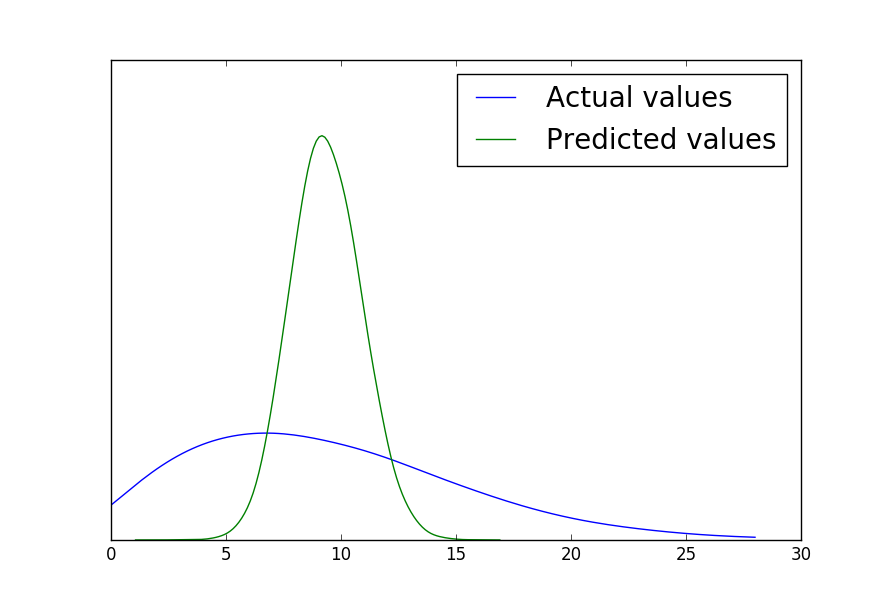
\includegraphics[scale=0.5]{predicted_assists}
\caption{Distribution of predicted values vs.\ actual variable distribution}
\label{fig:variablerange}
\end{figure}
During analysis of predictions produced by the prototype, I observed that the range of predictions was much smaller than the actual range for most variables.
An example of this can be seen on figure \ref{fig:variablerange}, where predictions rough range of 5 to 15, while actual variable range is roughly 0 to 30.
In addition, most of the machine learning techniques had similar predictive performance.
These two facts combined led me to believe that the problem is again with quality of features.
Therefore, I decided to create my own graphical model to generate richer features.
\section{Final System}
\subsection{Choosing distributions for variables}
\begin{figure}[ht]
\centering
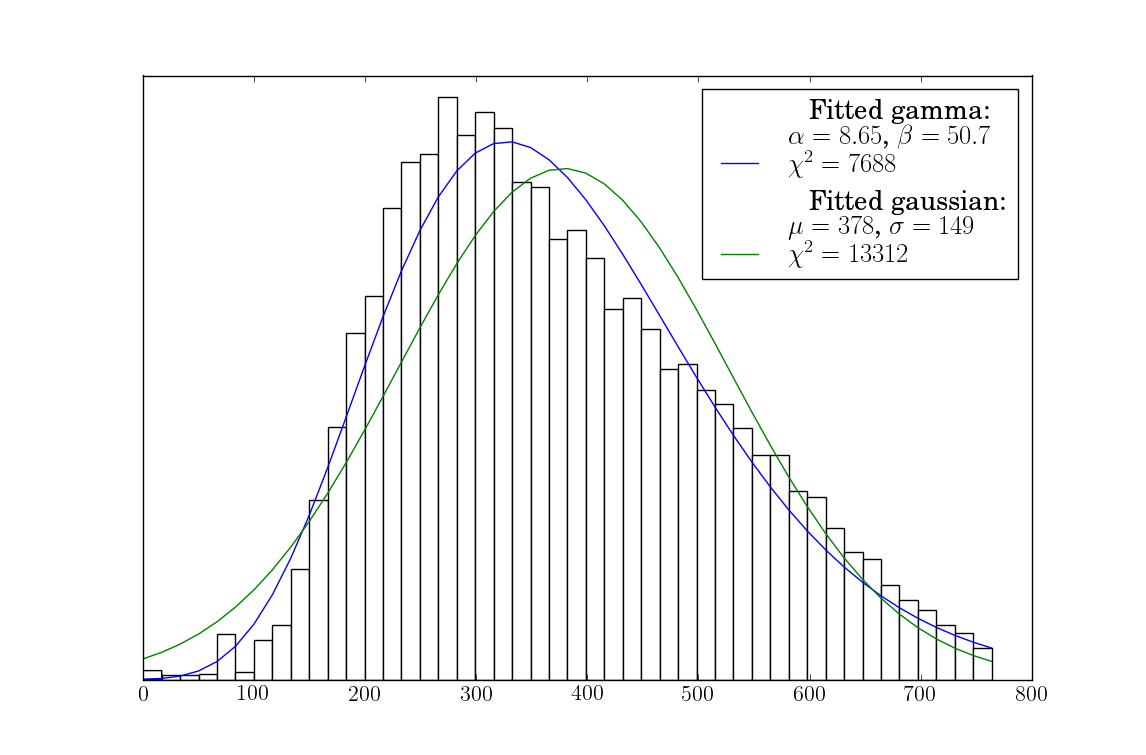
\includegraphics[scale=0.5]{fitted-distributions}
\caption{Fitted gaussian and gamma distributions on one of the variables.}
\note{Gamma distribution has a lower $\chi^2$ value, therefore it is a better fit.}
\label{fig:fitted-distributions}
\end{figure}
When predicting the values for each variable, rather than predicting the probability for each value independently, it is better to use a distribution to predict the probabilities for all values.
To decide which distribution fits each variable best, I used \emph{method of moments} to fit each potential distribution to all observed values of the variable.
Then I used \emph{goodness of fit} to decide which of the potential distributions is best.
\paragraph{Method of Moments}
To fit a distribution we need to estimate its parameters.
Parameters for most distributions can be easily expressed in terms of mean and variance of the data.
For example for Gamma distribution the equations are:
\begin{equation}
k= \mu^2/\sigma^2
\qquad
\theta = \sigma^2/\mu
\end{equation}
\paragraph{Goodness of fit}
To estimate how well the distribution fits the data we can use chi-squared test to measure sum of differences between observed and expected outcome frequencies:
\begin{equation}
\chi^2 = \sum_{i=1}^{n} \frac{(O_i - E_i)^2}{E_i}
\end{equation}
Where $O_i$ is the observed frequency and $E_i$ is the expected frequency.
\subsection{Player skills}
Every game is different and trying to pick specific set of skills for each one, would not be practical.
Therefore, I decided to make an assumption that players skill in a game can be described by $n$ real numbers.
Such $n$ will be different for each game and therefore is a hyper parameter in my model.
Since the system can never be sure on the exact skill values for each player, skills of each player are represented as $n$ Gaussian distributions.
\subsection{Neural networks}

\subsection{System overview}
\begin{figure}[ht]
\centering
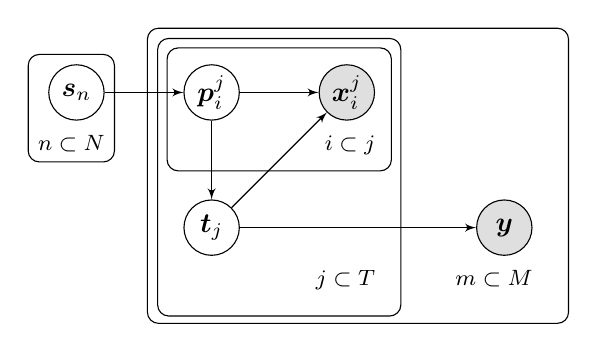
\begin{tikzpicture}
\tikzset{edge/.style = {->,> = latex'}}
\node[latent] (p) [] {$\bs{p}_i^j$};

\node[latent] (t) [below=of p] {$\bs{t}_j$};
\draw[edge] (p) to (t);

\node[obs] (x) [right=of p] {$\bs{x}_i^j$};
\draw[edge] (p) to (x);
\draw[edge] (t) to (x);

\node[obs] (y) [right=3cm of t] {$\bs{y}$};
\draw[edge] (t) to (y);

\plate[inner sep=0.2cm] {i} {(p)(x)} {$i\subset j$};
\plate[inner sep=0.32cm] {j} {(p)(x)(t)} {$j\subset T$};
\plate[inner sep=0.45cm] {m} {(p)(x)(t)(y)} {$m\subset M$};

\node[latent] (s) [left=of p] {$\bs{s}_n$};
\draw[edge] (s) to (p);
\plate {n} {(s)} {$n\subset N$};
\end{tikzpicture}
\caption{Summed up view of the prediction model.}
\note{There are $N$ players tracked by the system, participating in $M$ matches.
In each match there are $T$ teams.
$\bs{x}_i^j$ are the results of player $i$ in team $j$ and $\bs{y}$ are the overall match results.
Variables in bold are vectors.}
\label{fig:model-simple}
\end{figure}
The model assumes that there are two types of results for each game:
\begin{itemize}
\item Player specific results, such as amount of gold earned or number of enemies killed.
\item Overall game results, such as which team won or how long the game took.
\end{itemize}
The model further assumes that player specific results depend on skills of the relevant player and skills of every team, and overall results only depend on skills of each team.
This dependencies are seen in figure \ref{fig:model-simple}.
An example of a system made for a game in which four players play in two teams can be seen in figure \ref{fig:four-player-model}.

There are two parts in the system: predicting results from inferred player skills and inferring player skills from their history.
Training both the inner model for statistic prediction and model for player skill updates at the same time would greatly increase the data required for processing. %TODO check this
It will also raise some difficult problem such as \emph{vanishing gradient}, unfortunately I did not have enough time to solve them properly.
Instead I decided to use the technique called \emph{coordinate descent}, to optimise the models alternatively.
\paragraph{Coordinate descent}
When we have multiple parameters to optimise, instead of optimising them at the same time we can optimise them alternatively.
We optimise each parameter for a certain number of iterations (or until some criteria is achieved) and then move onto the next parameter.
Once we optimised each parameter, we can loop back and start again from the first one.
We do that until all parameters reach sufficiently stable values.
\begin{figure}[ht]
\centering
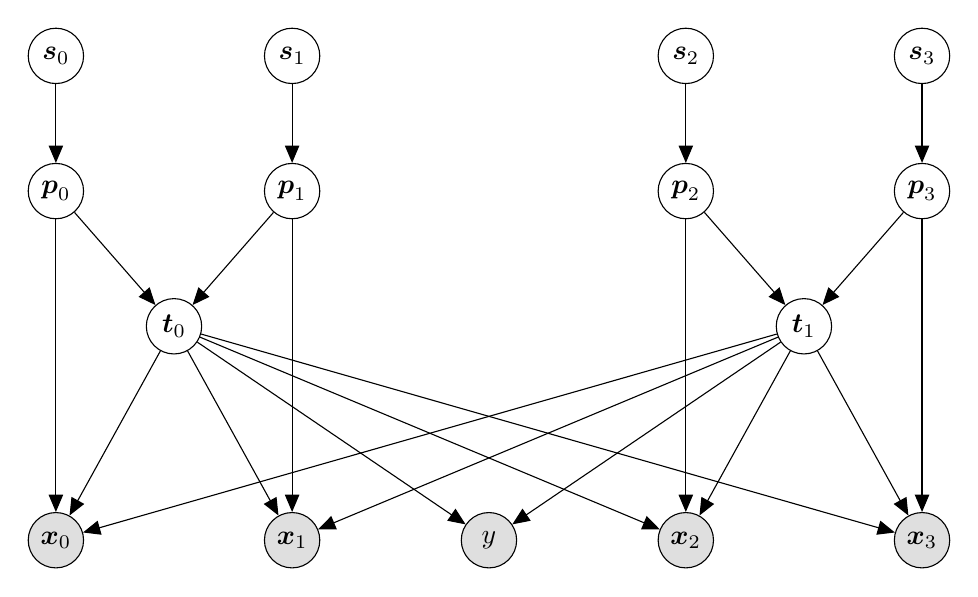
\begin{tikzpicture}
	% Team results
	\node[obs] (y) [] {$y$};	
	
	% Team performances
	\node[latent] (t0)[above=2cm of y, xshift=-4cm] {$\boldsymbol{t}_0$};
	\node[latent] (t1)[above=2cm of y, xshift=4cm] {$\boldsymbol{t}_1$};
	
	% Player results
 	\node[obs] (x0)[below= 2cm of t0, xshift=-1.5cm] {$\boldsymbol{x}_0$};
 	\node[obs] (x1)[below= 2cm of t0, xshift=1.5cm] {$\boldsymbol{x}_1$};
 	\node[obs] (x2)[below= 2cm of t1, xshift=-1.5cm] {$\boldsymbol{x}_2$};
 	\node[obs] (x3)[below= 2cm of t1, xshift=1.5cm] {$\boldsymbol{x}_3$};
 	
 	% Player performances
 	\node[latent] (p0)[above=of t0, xshift=-1.5cm] {$\boldsymbol{p}_0$};
 	\node[latent] (p1)[above=of t0, xshift=1.5cm] {$\boldsymbol{p}_1$};
 	\node[latent] (p2)[above=of t1, xshift=-1.5cm] {$\boldsymbol{p}_2$};
 	\node[latent] (p3)[above=of t1, xshift=1.5cm] {$\boldsymbol{p}_3$};
 	
 	% Player skills
 	\node[latent] (s0)[above=of p0] {$\boldsymbol{s}_0$};
 	\node[latent] (s1)[above=of p1] {$\boldsymbol{s}_1$};
 	\node[latent] (s2)[above=of p2] {$\boldsymbol{s}_2$};
 	\node[latent] (s3)[above=of p3] {$\boldsymbol{s}_3$};
 	
 	% Skill to performace
 	\edge[] {s0} {p0};
 	\edge[] {s1} {p1};
 	\edge[] {s2} {p2};
 	\edge[] {s3} {p3};
 	
 	%Player to team performance
 	\edge[] {p0,p1} {t0};
 	\edge[] {p2,p3} {t1};
 	
 	%Player results
 	\edge[] {p0,t0,t1} {x0};
 	\edge[] {p1,t0,t1} {x1};
 	\edge[] {p2,t1,t0} {x2};
 	\edge[] {p3,t1,t0} {x3};
 	
 	%Team performance
 	\edge[] {t0,t1} {y};
 	
	
\end{tikzpicture}
\caption{An example of an inference model for four players in two teams.}
\note{Grey circles represent observed values and white circles represent latent variables.}
\label{fig:four-player-model}
\end{figure}

%\begin{figure}[h]
%\centering
%\begin{tikzpicture}
%\tikzstyle{main}=[circle, thick, draw =black!80]
%\tikzstyle{connect}=[-latex, thick]
%\tikzstyle{box}=[rectangle, draw=black!100]
%	
%	% Team results
%	\node[main,fill=black!15] (y) [] {$\boldsymbol{y}$};
%	
%	% Team performances
%	\node[main] (t0)[above=3cm of y, xshift=-4.5cm] {$\boldsymbol{t}_0$};
%	\node[main] (t1)[above=3cm of y, xshift=4.5cm] {$\boldsymbol{t}_1$};
%	
%	% Player results
% 	\node[main,fill=black!15] (x0)[below= 3cm of t0, xshift=-1.5cm] {$\boldsymbol{x}_0$};
% 	\node[main,fill=black!15] (x1)[below= 3cm of t0, xshift=1.5cm] {$\boldsymbol{x}_1$};
% 	\node[main,fill=black!15] (x2)[below= 3cm of t1, xshift=-1.5cm] {$\boldsymbol{x}_2$};
% 	\node[main,fill=black!15] (x3)[below= 3cm of t1, xshift=1.5cm] {$\boldsymbol{x}_3$};
% 	
% 	% Player performances
% 	\node[main] (p0)[above=of t0, xshift=-1.5cm] {$\boldsymbol{p}_0$};
% 	\node[main] (p1)[above=of t0, xshift=1.5cm] {$\boldsymbol{p}_1$};
% 	\node[main] (p2)[above=of t1, xshift=-1.5cm] {$\boldsymbol{p}_2$};
% 	\node[main] (p3)[above=of t1, xshift=1.5cm] {$\boldsymbol{p}_3$};
% 	
% 	% Player skills
% 	\node[main] (s0)[above=of p0] {$\boldsymbol{s}_0$};
% 	\node[main] (s1)[above=of p1] {$\boldsymbol{s}_1$};
% 	\node[main] (s2)[above=of p2] {$\boldsymbol{s}_2$};
% 	\node[main] (s3)[above=of p3] {$\boldsymbol{s}_3$};
% 	
% 	% Skill input
% 	\node[factor,label=$\mathcal{N}(\boldsymbol{s}_0;\boldsymbol{\mu}_0.\ \boldsymbol{\sigma}_0^2)$] ()[above=of s0] {}
% 		edge [] (s0);
% 	\node[factor,label=$\mathcal{N}(\boldsymbol{s}_1;\boldsymbol{\mu}_1.\ \boldsymbol{\sigma}_1^2)$] ()[above=of s1] {}
% 		edge [] (s1);
% 	\node[factor,label=$\mathcal{N}(\boldsymbol{s}_2;\boldsymbol{\mu}_2.\ \boldsymbol{\sigma}_2^2)$] ()[above=of s2] {}
% 		edge [] (s2);
% 	\node[factor,label=$\mathcal{N}(\boldsymbol{s}_3;\boldsymbol{\mu}_3.\ \boldsymbol{\sigma}_3^2)$] ()[above=of s3] {}
% 		edge [] (s3);
% 		
% 	% Skill to performance
% 	\node[factor, label=left:$\Theta(\bs{p}_0;\bs{s}_0)$] () [above=of p0] {}
% 		edge [] (s0)
% 		edge [] (p0);
% 	\node[factor, label=left:$\Theta(\bs{p}_1;\bs{s}_1)$] () [above=of p1] {}
% 		edge [] (s1)
% 		edge [] (p1);
% 	\node[factor, label=left:$\Theta(\bs{p}_2;\bs{s}_2)$] () [above=of p2] {}
% 		edge [] (s2)
% 		edge [] (p2);
% 	\node[factor, label=left:$\Theta(\bs{p}_3;\bs{s}_3)$] () [above=of p3] {}
% 		edge [] (s3)
% 		edge [] (p3);
% 		
% 	% Performance to team
% 	\node[factor, label=185:$\Phi(\bs{t}_0;\bs{p}_0.\ \bs{p}_1)$] () [above=of t0] {}
% 		edge [] (p0)
% 		edge [] (p1)
% 		edge [] (t0);
% 	\node[factor, label=185:$\Phi(\bs{t}_1;\bs{p}_2.\ \bs{p}_3)$] () [above=of t1] {}
% 		edge [] (p2)
% 		edge [] (p3)
% 		edge [] (t1);
% 		
% 	% Team results
% 	\node[factor, label=185:$\text{Bern}(\boldsymbol{p}_{\psi}(\boldsymbol{t}_0.\ \boldsymbol{t}_1))$] () [above=of y] {}
% 		edge [] (t0)
% 		edge [] (t1)
% 		edge [] (y);
% 	
% 	% Player results
% 	\node[factor, label=185:$\Gamma(\bs{x}_0;\bs{p}_0.\ \bs{t}_0.\ \bs{t}_1)$] () [above=of x0] {}
% 		edge [] (p0)
% 		edge [] (t0)
% 		edge [] (t1)
% 		edge [] (x0);
% 	\node[factor, label=185:$\Gamma(\bs{x}_1;\bs{p}_1.\ \bs{t}_0.\ \bs{t}_1)$] () [above=of x1] {}
% 		edge [] (p1)
% 		edge [] (t0)
% 		edge [] (t1)
% 		edge [] (x1);
% 	\node[factor, label=185:$\Gamma(\bs{x}_2;\bs{p}_2.\ \bs{t}_1.\ \bs{t}_0)$] () [above=of x2] {}
% 		edge [] (p2)
% 		edge [] (t0)
% 		edge [] (t1)
% 		edge [] (x2);
% 	\node[factor, label=185:$\Gamma(\bs{x}_3;\bs{p}_3.\ \bs{t}_1.\ \bs{t}_0)$] () [above=of x3] {}
% 		edge [] (p3)
% 		edge [] (t0)
% 		edge [] (t1)
% 		edge [] (x3);
% 		
% 	%Results
% 	\node[factor,label=below:$\mathbb{I} (x) $] ()[below=of x0] {}
% 		edge [] (x0);
% 	\node[factor,label=below:$\mathbb{I} (x) $] ()[below=of x1] {}
% 		edge [] (x1);
% 	\node[factor,label=below:$\mathbb{I} (x) $] ()[below=of x2] {}
% 		edge [] (x2);
% 	\node[factor,label=below:$\mathbb{I} (x) $] ()[below=of x3] {}
% 		edge [] (x3);
%	\node[factor,label=below:$\mathbb{I} (y) $] ()[below=of y] {}
% 		edge [] (y);
% 		
% 	\node[text width=9cm] (a0) [below=of y,yshift=-1cm] {$\Theta(\bs{p};\bs{s})=\mathcal{N}(\bs{p};\bs{\mu}_{\theta}(\bs{s}), \bs{\sigma}_{\theta}^2(\bs{s}))$};
% 	\node[text width=9cm] (a1) [below=of a0,yshift=1cm] {$\Phi(\bs{t};\bs{p}_i,\bs{p}_j)=\mathcal{N}(\bs{t};\bs{\mu}_{\phi}(\bs{p}_i,\bs{p}_j), \bs{\sigma}_{\phi}^2(\bs{p}_i,\bs{p}_j))$ };
% 	\node[text width=9cm] (a2) [below=of a1,yshift=1cm] {
% 	$\Gamma(\bs{x};\bs{p},\bs{t}_i,\bs{t}_j)=\text{gamma}(\bs{x};\bs{k}_{\gamma}(\bs{p},\bs{t}_i,\bs{t}_j), \bs{\theta}_{\gamma}(\bs{p},\bs{t}_i,\bs{t}_j))$ };
%\end{tikzpicture}
%\caption{Example of a factor graph.}
%\label{fig:four-player-model}
%\end{figure}



\subsection{Prediction model}
There are five variables in the model: $\bs{x},\bs{y},\bs{t},\bs{p},\bs{s}$.
To make predictions we would like to calculate $P(\bs{x})$ and $P(\bs{y})$.
We know the joint distribution over all variables $P(\bs{x},\bs{y},\bs{t},\bs{p},\bs{s})$ as well as $P(\bs{s})$.
For example, if if we would like to predict $P(\bs{x})$, normally we could integrate $\bs{y},\bs{t},\bs{p}$ and $\bs{s}$ out using sum rule:
\begin{equation}
P(\bs{x}) = \int\limits_{\bs{Y}} \int\limits_{\bs{T}} \int\limits_{\bs{P}}\int\limits_{\bs{S}} P(\bs{x},\bs{y},\bs{t},\bs{p},\bs{s})
\end{equation}
Unfortunately, since $\bs{t},\bs{p}$ and $\bs{s}$ are vectors this is infeasible.

Using our knowledge about dependencies in the system and product rule we can simplify this equation:
\begin{equation}
P(\bs{x},\bs{y},\bs{t},\bs{p},\bs{s}) = P(\bs{x}\mid\bs{y},\bs{t},\bs{p},\bs{s}) P(\bs{y},\bs{t},\bs{p},\bs{s})
\end{equation}
We know that $\bs{x}$ only depend on $\bs{t}$ and $\bs{p}$, from our assumptions.
Therefore we can drop $\bs{y}$ and $\bs{s}$ from the conditional probability:
\begin{equation}
P(\bs{x},\bs{y},\bs{t},\bs{p},\bs{s}) = P(\bs{x}\mid\bs{t},\bs{p}) P(\bs{y},\bs{t},\bs{p},\bs{s})
\end{equation}
By applying product rule further, we get:
\begin{equation}
P(\bs{x},\bs{y},\bs{t},\bs{p},\bs{s}) = P(\bs{x}\mid\bs{t},\bs{p}) P(\bs{t}\mid\bs{p}) P(\bs{p}\mid\bs{s}) P(\bs{s})
\end{equation}
%TODO Check how to separate this.
%\paragraph{Separation}
%Next we can pull out those probabilities out which 
%\begin{equation}
%P(\bs{x},\bs{y},\bs{t},\bs{p},\bs{s}) = P(\bs{x}\mid\bs{t},\bs{p}) P(\bs{t}\mid\bs{p})P(\bs{p}\mid\bs{s}) P(\bs{s})
%\end{equation}
\paragraph{Neural Networks}
Conditional probabilities such as $P(\bs{t}\mid \bs{p})$ are specific to every game and most likely very complex.
In such cases I use machine learning techniques to approximate there probabilities, since this is a probability of a vector given another vector, neural networks are the perfect candidate to use.
All of the variables in the model are defined using distributions, therefore neural networks must output the parameters of required distribution.
For example:
\begin{equation}
P(\bs{x} \mid \bs{p},\bs{t})=\text{gamma}(\bs{x};\bs{k_\gamma}(\bs{p},\bs{t}), \bs{\theta_\gamma}(\bs{p},\bs{t}))
\end{equation}
Where parameters $\bs{k_\gamma}$ and $\bs{\theta_\gamma}$ are outputs of a neural network with inputs $\bs{p}$ and $\bs{t}$ parametrised by $\bs{\gamma}$.
\paragraph{Variational Methods}
During the skill update phase, we generate expected player skills 
\paragraph{Training neural networks}
To train a neural network a loss function is required.
All of the outputs are probability distributions, therefore we can use the probability density function (pdf) of the chosen distribution.
The higher the pdf, the better the estimate, but loss function is minimised, therefore we need to negate the pdf to define loss.
For example a loss function for a Gaussian would be:
\begin{equation}
\text{loss}(x,\mu,\sigma) = -\frac{1}{\sqrt{2\sigma^2\pi}}e^{-\frac{(x-\mu)^2}{2\sigma^2}}
\label{eq:gaussian-loss}
\end{equation}
where $x$ is the desired value and $\mu$ \& $\sigma$ are estimated parameters.

\paragraph{Optimising loss function}
The loss function is defined across the whole system, therefore we need to multiply the pdf of all the distributions.
Multiplication is expensive, to improve performance of the system we can take the log of the product to turn it into a sum:
\begin{equation}
\text{loss} = \log\left(\prod_{p\subset P}p(x)\right) = \sum_{p\subset P}\log(p(x))
\end{equation}
This does not break the system, since all probabilities are positive and log is an increasing function.
By taking the log of different parts of pdf itself we can improve the efficiency even more, e.g. Gaussian from equation \ref{eq:gaussian-loss} becomes:
\begin{equation}
{loss}(x,\mu,\sigma) = \log(2\pi)/2+\log(\sigma)+\frac{(x-\mu)^2}{2\sigma^2}
\end{equation}
The optimising function can only change the parameters produced by the neural networks, therefore constants in the loss function do not matter and can be removed, leaving:
\begin{equation}
\text{loss}(x,\mu,\sigma) = \log(\sigma)+\frac{(x-\mu)^2}{2\sigma^2}
\end{equation}
\paragraph{Restricting the range of the output}
Some of the parameters have to fall within certain range.
The most obvious way to achieve this, is to just clip the output values to the required range.
Unfortunately, by clipping values we restrict the ability of neural networks to learn, because clipping information is not passed to optimisation algorithm.
Instead we can use some function transforms to map the output values onto the required range.
To map real numbers onto positive reals (e.g. for standard deviation) we can use an exponential:
\begin{equation}
x' = e^x
\end{equation}
To map real numbers to values between zero and one (e.g. for probability of winning) we can use a logistic function:
\begin{equation}
x' = \frac{1}{1+e^{-x}}
\end{equation}

\subsection{Skill update model}

\subsection{Prediction}
To predict the values for a particular match-up we just need to take the set of skills corresponding to players in the match-up and feed them into the top of the model.

\paragraph{Restricting the time frame of training data}
Many popular multiplayer computer games change their rules a few times a year to keep the game fresh and players interested as well as to balance the irregularities.
In addition the strategies players employ evolve through time and different skills become more or less important in the game.
If the system is trained on the whole history of games, it is optimised to predict results across the whole time-frame, but most of the time we are only interested in predicting future results.
Therefore, to improve the accuracy of the system we can only use recent matches in which players employ current strategies to train the system.
Although, there is a trade-off: the smaller the time-frame the fewer matches are available for analysis.



\chapter{Evaluation}
\section{Preprocessing}
When neural networks have been trained, we need process every match in chronological order to update the player skills.
To make evaluation quicker we can create a dictionary which contains match id as keys and skills of the players taking part in that match.
We need to store the player skills before processing the match and updating them to accurately reflect real world scenario.
\section{Train/Validation/Test split}
One of the most important rules when evaluating machine learning systems is that the algorithm must be tested on previously unseen data.
Therefore right at the start we can split our data into two parts: \emph{train/validation} and \emph{test}.
\emph{Train/validation} set will be used to train the algorithm and adjust hyper-parameters.
\emph{Test} set will be used for evaluation of the algorithm.

To adjust hyper-parameters fairly we need to reflect evaluation procedure during our training.
For that purpose the train/validation set is further split into two parts: \emph{train} and \emph{validation}.
\subsection{Cross-validation}
If we reuse the same part for validation, we run the risk of over-fitting our algorithm to that particular part of the dataset.
To combat that, we can use cross-validation: we run train/validation multiple times, each time picking new set to use for validation.
To ensure complete coverage of the train-set we can use \emph{k-fold cross-validation}: 
\begin{enumerate}
\item Divide the training set into $k$ random subsets.
\item Pick a subset that has not been validated on, use it for validation and the rest for training.
Record the result.
\item Repeat step two until all subsets have been used for validation.
\item Average the results.
\end{enumerate}


\chapter{Conclusions}


\printbibliography[heading=bibintoc,title={Bibliography}]

\appendix
\chapter{Example of a Statistic} \label{statexample}
Some parts of this statistic are repetetive and take up a lot of space.
In such parts, all but the first set were hidden, indicated by comments in $<>$.
\begin{lstlisting}[language=json,firstnumber=1, basicstyle=\small]
{  
   "result":{  
      "players":[  
         {  
            "account_id":87382579,
            "player_slot":0,
            "hero_id":60,
            "item_0":239,
            "item_1":92,
            "item_2":46,
            "item_3":108,
            "item_4":29,
            "item_5":6,
            "backpack_0":0,
            "backpack_1":0,
            "backpack_2":0,
            "kills":3,
            "deaths":7,
            "assists":17,
            "leaver_status":0,
            "last_hits":72,
            "denies":2,
            "gold_per_min":254,
            "xp_per_min":298,
            "level":14,
            "hero_damage":5682,
            "tower_damage":277,
            "hero_healing":170,
            "gold":73,
            "gold_spent":9220,
            "scaled_hero_damage":0,
            "scaled_tower_damage":0,
            "scaled_hero_healing":0,
            "ability_upgrades":[  
               {  
                  "ability":5275,
                  "time":886,
                  "level":1
               },
               <There is one set per level and players can advance up to level 25>
            ]
         },
         <There are nine more sets of player data>
      ],
      "radiant_win":false,
      "duration":2368,
      "pre_game_duration":90,
      "start_time":1471142574,
      "match_id":2569610900,
      "match_seq_num":2244488581,
      "tower_status_radiant":1540,
      "tower_status_dire":1956,
      "barracks_status_radiant":3,
      "barracks_status_dire":63,
      "cluster":113,
      "first_blood_time":89,
      "lobby_type":1,
      "human_players":10,
      "leagueid":4664,
      "positive_votes":38429,
      "negative_votes":2503,
      "game_mode":2,
      "flags":1,
      "engine":1,
      "radiant_score":27,
      "dire_score":30,
      "radiant_team_id":2512249,
      "radiant_name":"Digital Chaos",
      "radiant_logo":692780106202747975,
      "radiant_team_complete":1,
      "dire_team_id":1836806,
      "dire_name":"the wings gaming",
      "dire_logo":352770708597344369,
      "dire_team_complete":1,
      "radiant_captain":87382579,
      "dire_captain":111114687,
      "picks_bans":[  
         {  
            "is_pick":false,
            "hero_id":79,
            "team":1,
            "order":0
         },
         <There are about 20 sets in this list, detailing the drafting phase>
      ]
   }
}
\end{lstlisting}

\chapter{Project Proposal}

\end{document}
